\documentclass[12pt, a4paper]{exam}
\usepackage{graphicx}
\usepackage[left=0.8in, top=0.7in, total={6.2in,8in}]{geometry}
\usepackage[normalem]{ulem}
\renewcommand\ULthickness{1.0pt}   %%---> For changing thickness of underline
\setlength\ULdepth{1.3ex}%\maxdimen ---> For changing depth of underline

\begin{document}
	%\thispagestyle{empty}
	\noindent
	\begin{minipage}[l]{0.1\textwidth}
		\noindent
		
\includegraphics[width=2.4\textwidth]{logo.png}
	\end{minipage}
	\hfill

\begin{minipage}[c]{0.8\textwidth}
	\begin{center}
		{\large Universidad La Salle \par
		\small Ingeniería de Sofware	\par
		\large Fundamentos de Lenguajes de Programación	\par
\small Karlo Pacha Curimayhua \par
\small Fecha: Octubre 25, 2022} \par
	\end{center}
\end{minipage}
\par
\vspace{0.2in}
\noindent
\par 
\vspace{0.15in}
\noindent
\centering { \small \bfseries Práctica 13 } \par
\centering { \small \ Ejercicios }


%q1
\begin{questions}
	\pointsdroppedatright
	\question Investigue el concepto de first class en Javascript y muestre una pequeña defición seguida ejemplos. (2 puntos)
	\begin{parts}
		\part Son funciones que son tratadas como cualquier otra variable; estas puedes ser pasadas como argumento a otras funciones, puede ser retornada por otra función y puede ser asignada a una variable.
	\end{parts}
\vspace{0.2in}

\begin{verbatim}
	const Arithmetics = {
		add: (a, b) => {
			return `${a} + ${b} = ${a + b}`;
		},
		subtract: (a, b) => {
			return `${a} - ${b} = ${a - b}`
		},
		multiply: (a, b) => {
			return `${a} * ${b} = ${a * b}`
		},
		division: (a, b) => {
			if (b != 0) return `${a} / ${b} = ${a / b}`;
			return `Cannot Divide by Zero!!!`;
		}
	}
\end{verbatim}


%q2
\pointsdroppedatright
	\question Describa la diferencia entre Currying and Partial Application. Incluya ejemplos. (2 puntos)
	\begin{parts}
		\part Currying: Una función que toma una función con múltiples parámetros como entrada y devuelve una función con exactamente un parámetro.
		\part Partial Application: El proceso de aplicar una función a algunos de sus argumentos. La función aplicada parcialmente se devuelve para su uso posterior. 
		\vspace{0.05in}
	\end{parts}
\vspace{0.2in}

\begin{verbatim}
	function partial(firstArgument, secondArgument) {
		return function(thirdArgument, fourthArgument, fifthArgument) {
			return firstArgument + secondArgument + thirdArgument + fourthArgument + fifthArgument;
		}
	}

	function curry(firstArgument) {
		return function(secondArgument) {
			return function(thirdArgument) {
				return function(fourthArgument ) {
					return function(fifthArgument) {
						return firstArgument + secondArgument + thirdArgument + fourthArgument + fifthArgument;
					}
				}
			}
		}
	}
\end{verbatim}

%q3
\pointsdroppedatright
	\question Implemente una función que calcule el volumen de un cilindro. Incluya la versión normal y una aplicando Currying. (2 puntos)
	\begin{verbatim}
		var NormalCylinderVolume = (r, h) => Math.PI * Math.pow(r,2) * h;

		console.log("Normal: ",NormalCylinderVolume(2, 3));

		var CurryingCylinderVolume =(r) => {
			return (h) => Math.PI * Math.pow(r,2) * h;
		}
		console.log("Currying: ",CurryingCylinderVolume(2)(3));
	\end{verbatim}

	\begin{figure}[h]
		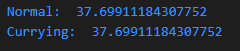
\includegraphics[width=8cm]{3.png}
	\end{figure}
\vspace{0.2in}

%q4
\pointsdroppedatright
	\question Cree una función joinWords que una varios parametros de tipo string. (3 puntos)
	\begin{verbatim}
		function joinWords(string1) {
			return (string2) => !string2 ? string1 : joinWords(`${string1} ${string2}`);
		}

		result = joinWords('Hello')();
		console.log(result); // Hello

		result = joinWords('There')('is')('no')('spoon.')();
		console.log(result); // There is no spoon.
	\end{verbatim}

	\begin{figure}[h]
		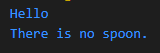
\includegraphics[width=8cm]{4.png}
	\end{figure}
\vspace{0.2in}

%q5
\pointsdroppedatright
	\question Implemente una función delayInvoc que en cada invocación incremente la variable total con el valor enviado como parametro. (3 puntos)
	\begin{verbatim}
		fvar total = 0;

		var delayInvoc = function (a) {
			total += a;
			return function (b) {        
				if(b) return delayInvoc(b);
			};
		};
		
		
		delayInvoc(4)(5);
		console.log("4,5: ",total); //9
		
		delayInvoc(4)(5)(8);
		console.log("4,5,8: ",total); // 26
		
		delayInvoc(1)(1)(1)(1);
		console.log("1,1,1,1: ",total); // 30
	\end{verbatim}

	\begin{figure}[h]
		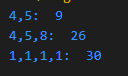
\includegraphics[width=8cm]{5.png}
	\end{figure}
\vspace{0.2in}

%q6
\pointsdroppedatright
	\question Implemente una función curry que tome como argumento cualquier función f y retorne la versión curried de f. (4 puntos)
	\begin{verbatim}
		function abc(a, b, c) {
			return a+b+c;
		}
		
		function curry(f) {
			return function curry2(...args) {
				if (args.length >= f.length) return f.apply(this, args);
				else return function curry3(...args2) {
					return curry2.apply(this, args.concat(args2));
				}
			};
		}
		  
		var curriedAbc = curry(abc);
		
		console.log("(2)(3)(4): ", curriedAbc(2)(3)(4)); // 9
		console.log("(2, 3)(4): ", curriedAbc(2, 3)(4)); // 9
		console.log("(2)(3, 4): ", curriedAbc(2)(3, 4)); // 9
		console.log("(2, 3, 4): ", curriedAbc(2, 3, 4)) ; // 9
	\end{verbatim}

	\begin{figure}[h]
		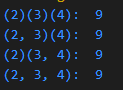
\includegraphics[width=8cm]{6.png}
	\end{figure}
\vspace{0.2in}

\large GitHub: 
\small https://github.com/KEPCU/FundamentalsOfProgrammingLanguages/tree/master/js/practice13
\end{document}